\chapter{Przegląd literatury}
Celem niniejszego rozdziału jest przedstawienie dotychczasowych badań i publikacji dotyczących mechanizmów programowania współbieżnego i równoległego w językach Rust i C++. Analiza literatury umożliwi zrozumienie aktualnego stanu wiedzy w tej dziedzinie, a także wskazanie na występujące luki badawcze, które niniejsza praca postara się wypełnić.
Na samym wstępie zostały postawione następujące pytania do przeglądu literatury, które pomogą zrozumieć oraz sprawdzić aktualny stan wiedzy jeżeli chodzi o porównanie języków Rust oraz C++:

\begin{quote}
    \item \textbf{PPL1:} \emph{Jakie główne koncepcje/teorie dominują w literaturze dotyczącej porównania języków Rust oraz C++?} \label{PPL1}
    \item \textbf{PPL2:} \emph{Jakie metody badawcze są najczęściej stosowane do analizy różnic pomiędzy językami?}
    \item \textbf{PPL3:} \emph{Jak wygląda porównanie dostępności i dojrzałości bibliotek do programowania współbieżnego i równoległego w obu językach?}
    \item \textbf{PPL4:} \emph{Czy istnieją systematyczne metodologie porównywania języków programowania w kontekście współbieżności, które można zastosować do analizy Rust i C++?}
    \item \textbf{PPL5:} \emph{Jakie aspekty programowania współbieżnego i równoległego w Rust i C++ nie zostały dostatecznie zbadane w literaturze?}
    \item \textbf{PPL6:} \emph{Jaki jest stan wiedzy na temat wykorzystania programowania współbieżnego w ramach GPU w językach Rust i C++?}
\end{quote}

Odpowiedzi na powyższe pytania pozwolą na zidentyfikowanie kluczowych obszarów, które wymagają dalszych badań oraz na wskazanie na potencjalne kierunki rozwoju w dziedzinie programowania współbieżnego i równoległego w językach Rust i C++.\\
\subsection{Metodologia przeglądu literatury}
Proces przeglądu literatury został zrealizowany zgodnie z zasadami przeglądu systematycznego, co oznaczało zastosowanie jasno określonych kryteriów selekcji i wyłączenia. Główne źródła literaturowe obejmowały artykuły naukowe, materiały konferencyjne oraz dokumentację techniczną. Wyszukiwanie przeprowadzono w renomowanych bazach danych naukowych oraz repozytoriach zawierających publikacje z zakresu inżynierii oprogramowania i języków programowania. Dodatkowo zostały również uwzględnione źródła internetowe oraz dokumentacje techniczne.\\
Przegląd literatury odbywał się z wykorzystaniem narzędzi baz danych oferujących wyszukiwanie, filtrowanie oraz przegląd prac: Scopus, Google Scholar.\\
\subsection{Baza Scopus}
W ramach bazy scopus wykorzystano następujące kwerendy do wyszukiwania - tabela \ref{table:literatureReviewQueries}

\begin{table}[H]
    \caption{Kwerendy użyte w bazie Scopus \protect \footnotemark}
    \label{table:literatureReviewQueries}
    \begin{tabular}{|c|p{11cm}|c|}
    \hline
    Lp. & Kwerenda & Liczba wyników \\ \hline
    1 & ALL ("concurrent programming"\ OR "parallel programming") AND (ALL ("Rust") AND ALL ("C++")) & 444 \\ \hline

    2 & ALL ("concurrent programming"\ OR "parallel programming") AND (ALL ("Rust") AND ALL ("C++") ) AND ( ALL ("compare")) & 28 \\ \hline

    3 & (TITLE-ABS-KEY(("concurrent programming"\ OR "parallel programming") AND ("Rust"\ AND "C++"))) AND (TITLE-ABS-KEY("comparison"\ OR "evaluation"\ OR "benchmark")) & 6 \\ \hline

    4 & (TITLE-ABS-KEY(("thread"\ OR "async"\ OR "future"\ OR "actor model"\ OR "message passing"\ OR "shared memory") AND ("Rust"\ AND "C++"))) AND (TITLE-ABS-KEY("comparison"\ OR "performance"\ OR "evaluation")) & 50 \\ \hline

    5 & (TITLE-ABS-KEY(("Rust"\ AND "C++") AND ("concurrency model"\ OR "parallel constructs"\ OR "multithreading"))) AND (TITLE-ABS-KEY("comparison"\ OR "study")) & 2 \\ \hline

    \end{tabular}
\end{table}
\footnotetext{Ilość wyników dla poszczególnych zapytań może się różnić w zależności od daty (wyszukiwanie przeprowadzono w okresie listopad-luty 2024/25).}

W celu identyfikacji literatury związanej z porównaniem wybranych mechanizmów programowania współbieżnego i równoległego w językach Rust i C++, opracowano pięć zapytań w bazie Scopus, z których każde miało określony cel badawczy. Pierwsze zapytanie miało na celu uzyskanie ogólnego przeglądu literatury, wyszukując wszystkie dokumenty, w których występują jednocześnie zagadnienia programowania współbieżnego lub równoległego oraz języki Rust i C++, niezależnie od kontekstu. Pozwoliło to oszacować ogólną skalę badań łączących te zagadnienia. Drugie zapytanie zawężało zakres wyszukiwania poprzez dodanie słowa kluczowego „compare”, co umożliwiło wyodrębnienie publikacji, w których dokonano bezpośredniego porównania języków Rust i C++ w kontekście współbieżności lub równoległości. Dzięki temu uzyskano bardziej ukierunkowany zbiór literatury odnoszącej się do analizy porównawczej. Trzecie zapytanie charakteryzowało się większą precyzją, ograniczając wyniki do tytułów, streszczeń oraz słów kluczowych, i uwzględniało wyłącznie publikacje zawierające odniesienia do ewaluacji, porównań bądź benchmarków języków Rust i C++. Takie podejście pozwoliło wyselekcjonować najbardziej tematycznie powiązane prace. Czwarte zapytanie miało charakter bardziej techniczny, koncentrując się na konkretnych mechanizmach współbieżności, takich jak wątki, asynchroniczność, obiekty typu futury, model aktorów, przesyłanie komunikatów czy pamięć współdzielona, w połączeniu z terminami dotyczącymi wydajności i oceny. Umożliwiło to dotarcie do badań analizujących niskopoziomowe aspekty działania tych mechanizmów w obu językach. Piąte zapytanie skupiało się na poziomie koncepcyjnym, wyszukując publikacje zawierające takie terminy jak model współbieżności, konstrukty równoległe czy wielowątkowość, wraz z frazami dotyczącymi porównań lub analiz. Celem było zidentyfikowanie prac badających różnice w podejściu do współbieżności na poziomie architektury języka i jego konstrukcji wewnętrznych.

Autor zdecydował się również użyć nowego, wbudowane narzędzia w systemie Scopus - Scopus AI. Narzędzie to oparte na sztucznej inteligencji, wspomaga eksplorację akademicką w oparciu o dane z platformy Scopus. Dzięki integracji z narzędziem Copilot optymalizuje wyszukiwania, łącząc metody semantyczne i dopasowanie słów kluczowych. Choć Scopus AI ułatwia badania, jego wyniki warto weryfikować, ponieważ mogą zawierać nieścisłości lub stronniczość. \\
Po wprowadzeniu tytułu pracy w języku angielskim jako kwerendę, Scopus AI zwrócił 9 wyników, biorąc pod uwagę kwerendę stworzoną na podstawie tytyułu pracy, zamieszczoną w listingu \ref{AIQuery}. Zwrócone prace pokrywają się z przeglądem umieszczonym w tabeli \ref{table:literatureReviewQueries} 

\lstset{breaklines=true}
\begin{lstlisting}[caption=Kwerenda wygenerowana przez AI, label=AIQuery]
("concurrent programming" OR "parallel programming" OR "multithreading" OR "asynchronous")
AND ("Rust" OR "C++" OR "programming languages" OR "software development")
AND ("performance" OR "efficiency" OR "scalability" OR "resource management")
AND ("synchronization" OR "thread safety" OR "deadlock" OR "race condition")
AND ("libraries" OR "frameworks" OR "tools" OR "APIs")
\end{lstlisting}

\subsection{Kryteria selekcji oraz wyłączenia}
W procesie selekcji literatury uwzględniano przede wszystkim publikacje wydane po 2012 roku, co wynika z faktu, iż w tym właśnie roku zadebiutował język Rust \cite{wikipediaRustprogramming}. Wyjątek stanowiły prace o charakterze ogólnym lub takie, które nie odnosiły się bezpośrednio do języka Rust, lecz zawierały istotne informacje dla problematyki badawczej niniejszej pracy.

Analiza obejmowała literaturę w języku polskim oraz angielskim, przy czym zdecydowana większość źródeł stanowiły publikacje anglojęzyczne. Selekcja materiałów opierała się na zgodności tematycznej z zakresem badań. W przypadku wątpliwości co do adekwatności danej pozycji, decyzja o jej włączeniu do przeglądu podejmowana była na podstawie analizy streszczenia. Jeśli po tej analizie publikacja wydawała się istotna, przechodzono do pełnej oceny jej treści.

Publikacje, które po dogłębnej analizie okazywały się nieodpowiednie dla głównego problemu badawczego, nie były uwzględniane w zasadniczej części pracy. Niemniej jednak, jeśli przyczyniły się do lepszego zrozumienia badanego zagadnienia lub pomogły w odpowiedzi na pytania do przeglądu literatury \ref{PPL1}, były one odnotowywane jako materiały pomocnicze. Prace niespełniające powyższych kryteriów lub te, które nie są dostępne za pośrednictwem dostępnych metod (bądź też braku odpowiedzi twórców o prośbę udostępnienia pracy) były wykluczane z dalszej analizy.

\section{Porównanie Rust oraz C++}
Porównanie języków programowania Rust i C++ jest przedmiotem licznych publikacji, które analizują ich różnorodne aspekty, takie jak struktura kodu, sposób kompilacji, bezpieczeństwo, wydajność oraz obsługa współbieżności i równoległości. Niestety wśród prac naukowych zidentyfikowanych w bazach danych Scopus oraz Google Scholar, nie znaleziono prac, które jednoznacznie porównywałyby oba języki w kontekście programowania współbieżnego i równoległego.\\
W literaturze można znaleźć prace, które analizują różnice między Rustem a C++ w kontekście bezpieczeństwa, wydajności, zarządzania pamięcią oraz obsługi błędów.

\subsection{Bezpieczeństwo}
\label{Bezpieczeństwo}
Bezpieczeństwo języków Rust i C++ jest jednym z najczęściej analizowanych tematów w literaturze. W przypadku Rusta duży nacisk kładziony jest na eliminację całych klas błędów, takich jak null pointer dereferencing, data races oraz wycieki pamięci. Mechanizmy takie jak ownership, borrow checker oraz obowiązkowa mutowalność zmiennych (explicit mutability) są wymieniane jako kluczowe elementy zapewniające bezpieczeństwo oraz minimalizując ryzyko wycieków pamięci \cite{MigratingCtoRustforMemorySafety}. 

Z drugiej strony, C++ umożliwia większą kontrolę nad pamięcią, co może być zaletą w systemach wymagających maksymalnej wydajności, ale jednocześnie wiąże się z koniecznością samodzielnego zarządzania zasobami przez programistów. W literaturze \cite{RustDifferences, RustDifferences1} często podkreśla się, że to właśnie większa złożoność i ryzyko błędów w kodzie C++ skłoniły społeczność do stworzenia języków takich jak Rust.

Przykładowo, badania \cite{RustSafety1, RustSafety2, RustSafety3} wskazują, że aplikacje napisane w Rusta są mniej podatne na błędy związane z wyścigami danych \eng{data races}, co ma szczególne znaczenie w środowiskach wielowątkowych. Z kolei w C++ stosowanie bibliotek takich jak std::thread czy frameworków typu OpenMP pozwala na osiągnięcie podobnych celów, choć wymaga od programistów większej uwagi w zakresie synchronizacji. Dodatkowo są również prace \cite{PPL1_1,PPL1_2}, które przedstawiają próby implementacji mechanizmów wbudowanych w język Rust (prawo własności, pożyczka) do języka C.
\subsection{Czas wykonania}
\label{CzasWykonania}
Porównania czasów wykonania programów napisanych w Rust i C++ są częstym tematem analiz \cite{RustPerformance1, RustPerformance2, RustPerformance3, RustPerformance4}. W badaniach tych zostało wykazane, że pod względem wydajności Rust jest konkurencyjny wobec C++, co wynika z mechanizmów kompilacji i optymalizacji kodu.

Jednak kluczową różnicą jest to, że Rust wprowadza pewne narzuty związane z kontrolą bezpieczeństwa w czasie kompilacji, które mogą wydłużyć czas budowania programu, ale nie wpływają znacząco na czas wykonania.\\
Rust i C++ są językami kompilowanymi, co oznacza, że dedykowany kompilator tłumaczy kod źródłowy na kod maszynowy przed jego wykonaniem. Dzięki temu możliwe jest uzyskanie wysokiej wydajności programów. W literaturze \cite{Lesiński} często podkreśla się, że Rust, w odróżnieniu od C++, kładzie większy nacisk na bezpieczeństwo pamięci oraz typów w czasie kompilacji, co ma kluczowe znaczenie w nowoczesnym oprogramowaniu. W kontekście C++ wskazuje się na jego większą elastyczność oraz bogaty ekosystem, który pozwala na szeroką gamę zastosowań, ale jednocześnie wymaga większej uwagi programistów w zakresie zarządzania pamięcią i synchronizacji wątków.
% two images next to each other
\begin{figure}[H]
    \centering
    \begin{minipage}{.5\textwidth}
        \centering
        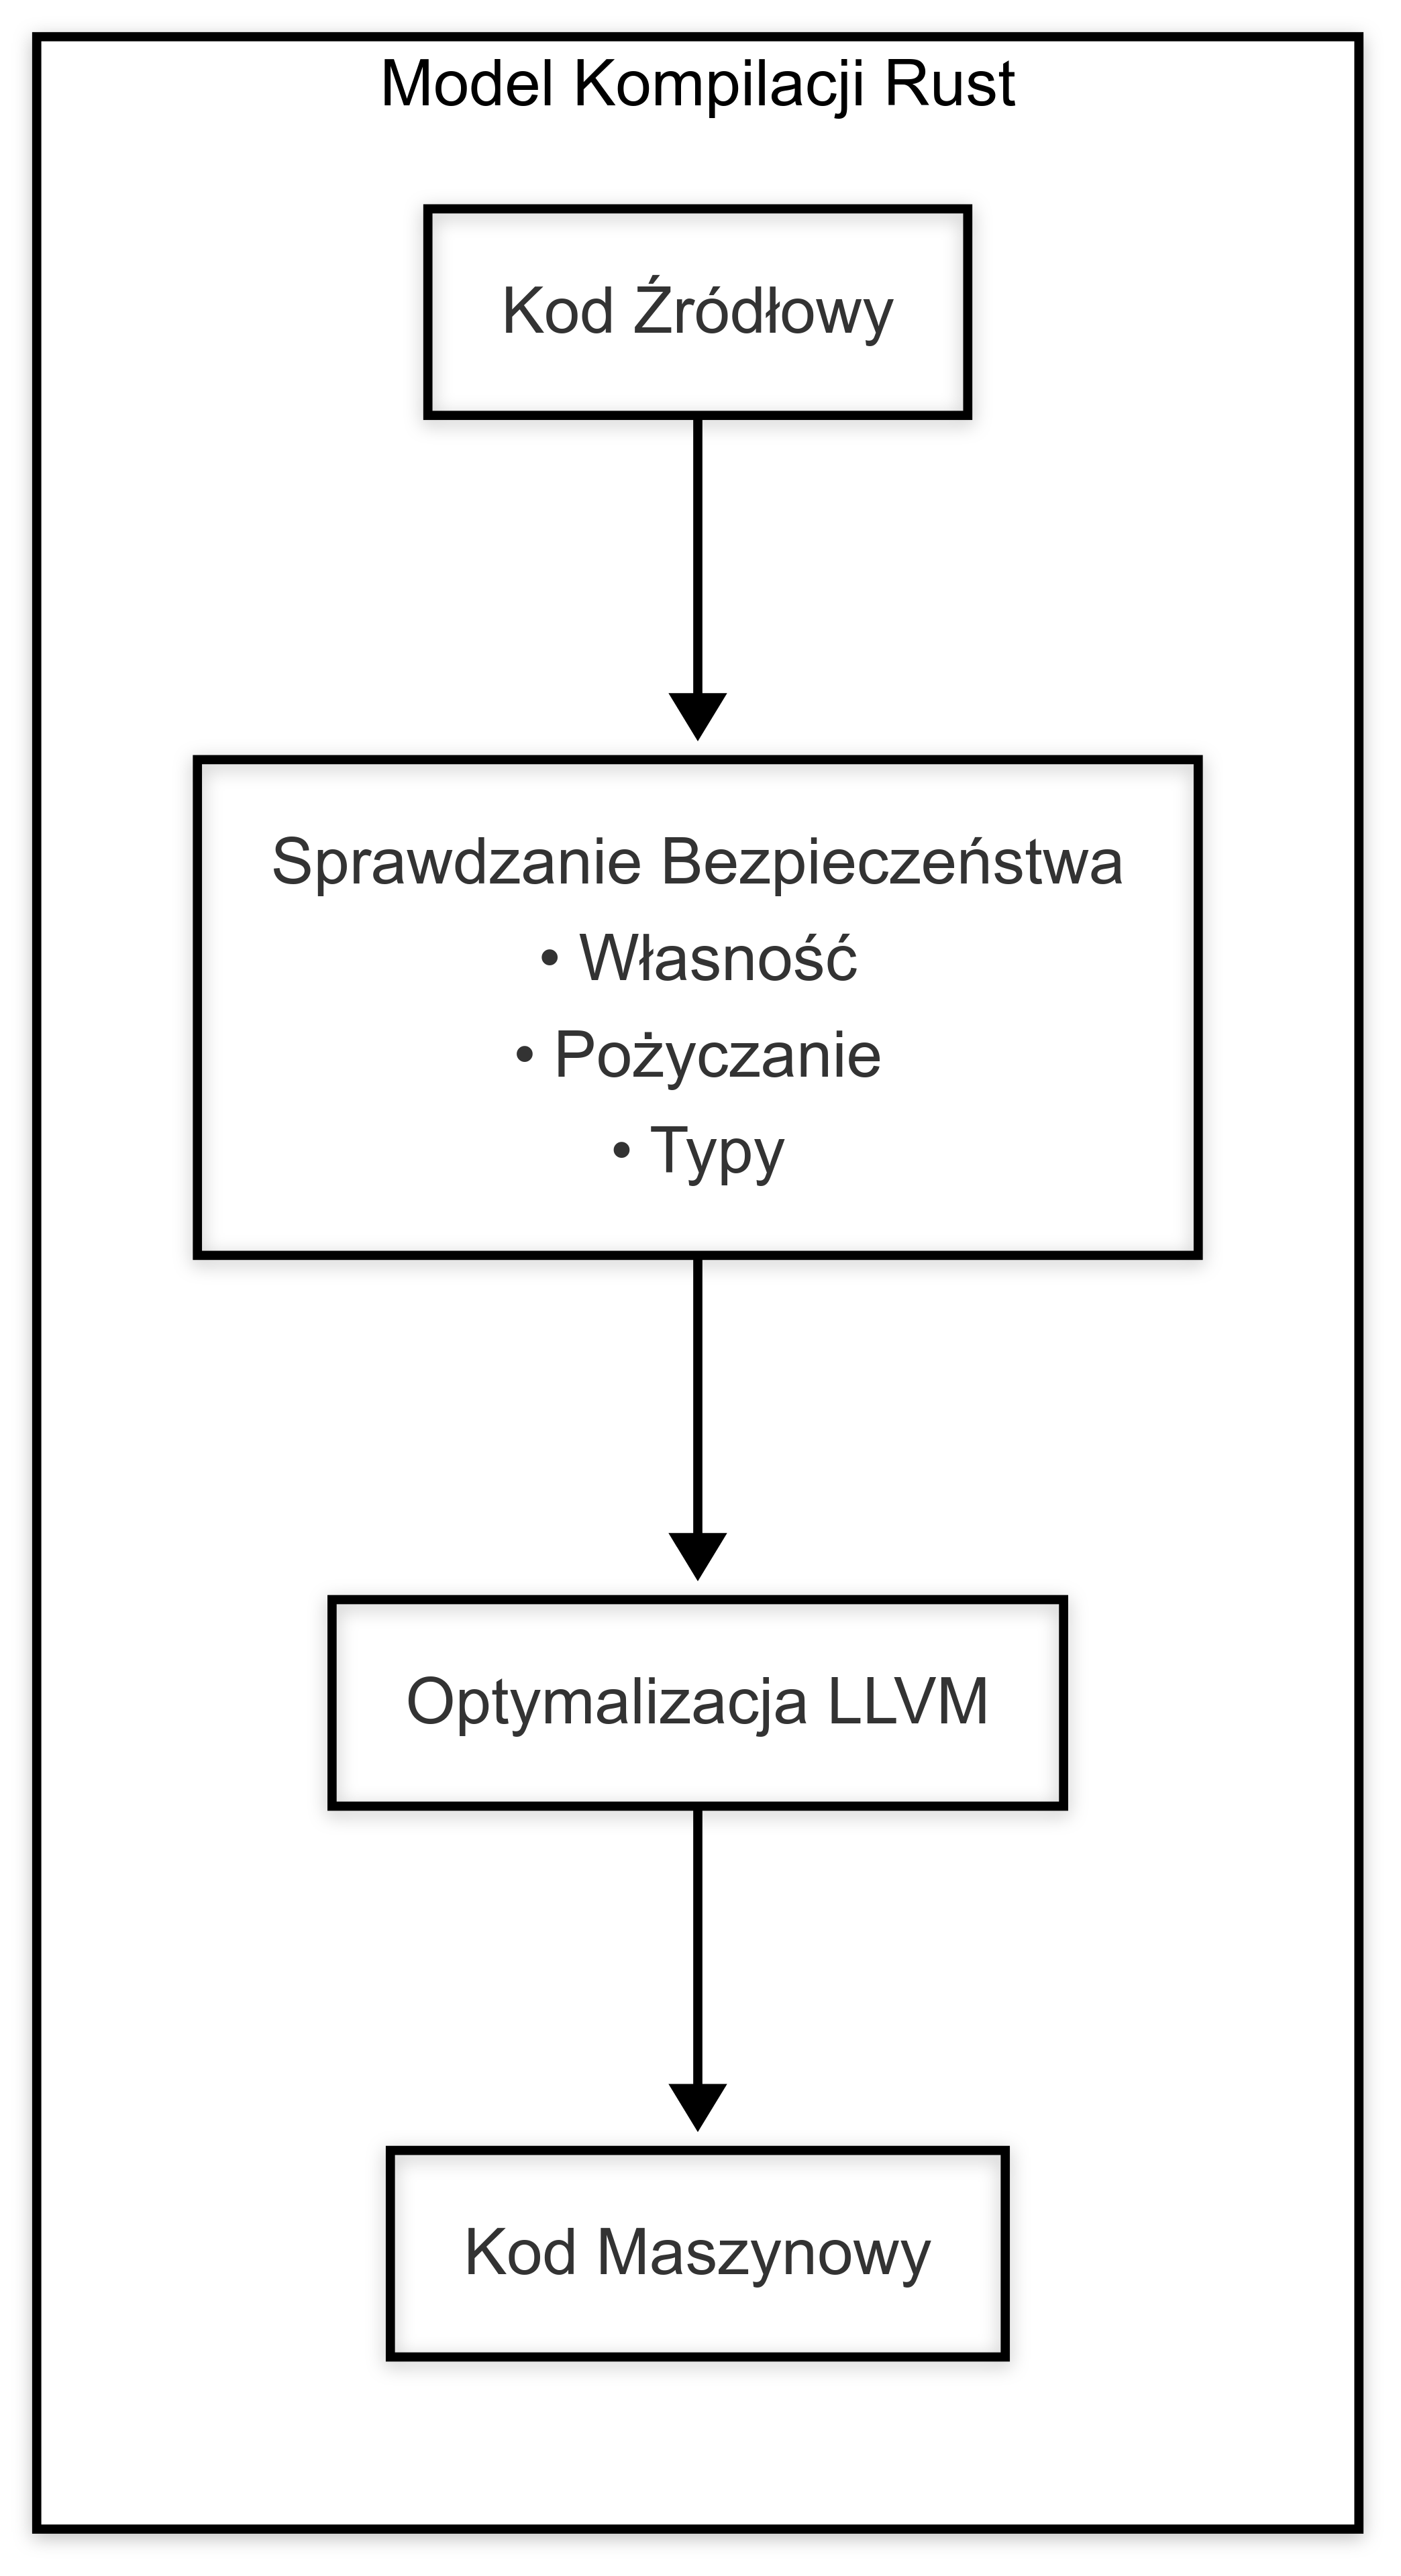
\includegraphics[height=12cm]{images/RustBuildsSteps.png}
        \caption{Kroki kompilacji w języku Rust}
        \label{fig:rust_build_steps}
    \end{minipage}%
    \begin{minipage}{.5\textwidth}
        \centering
        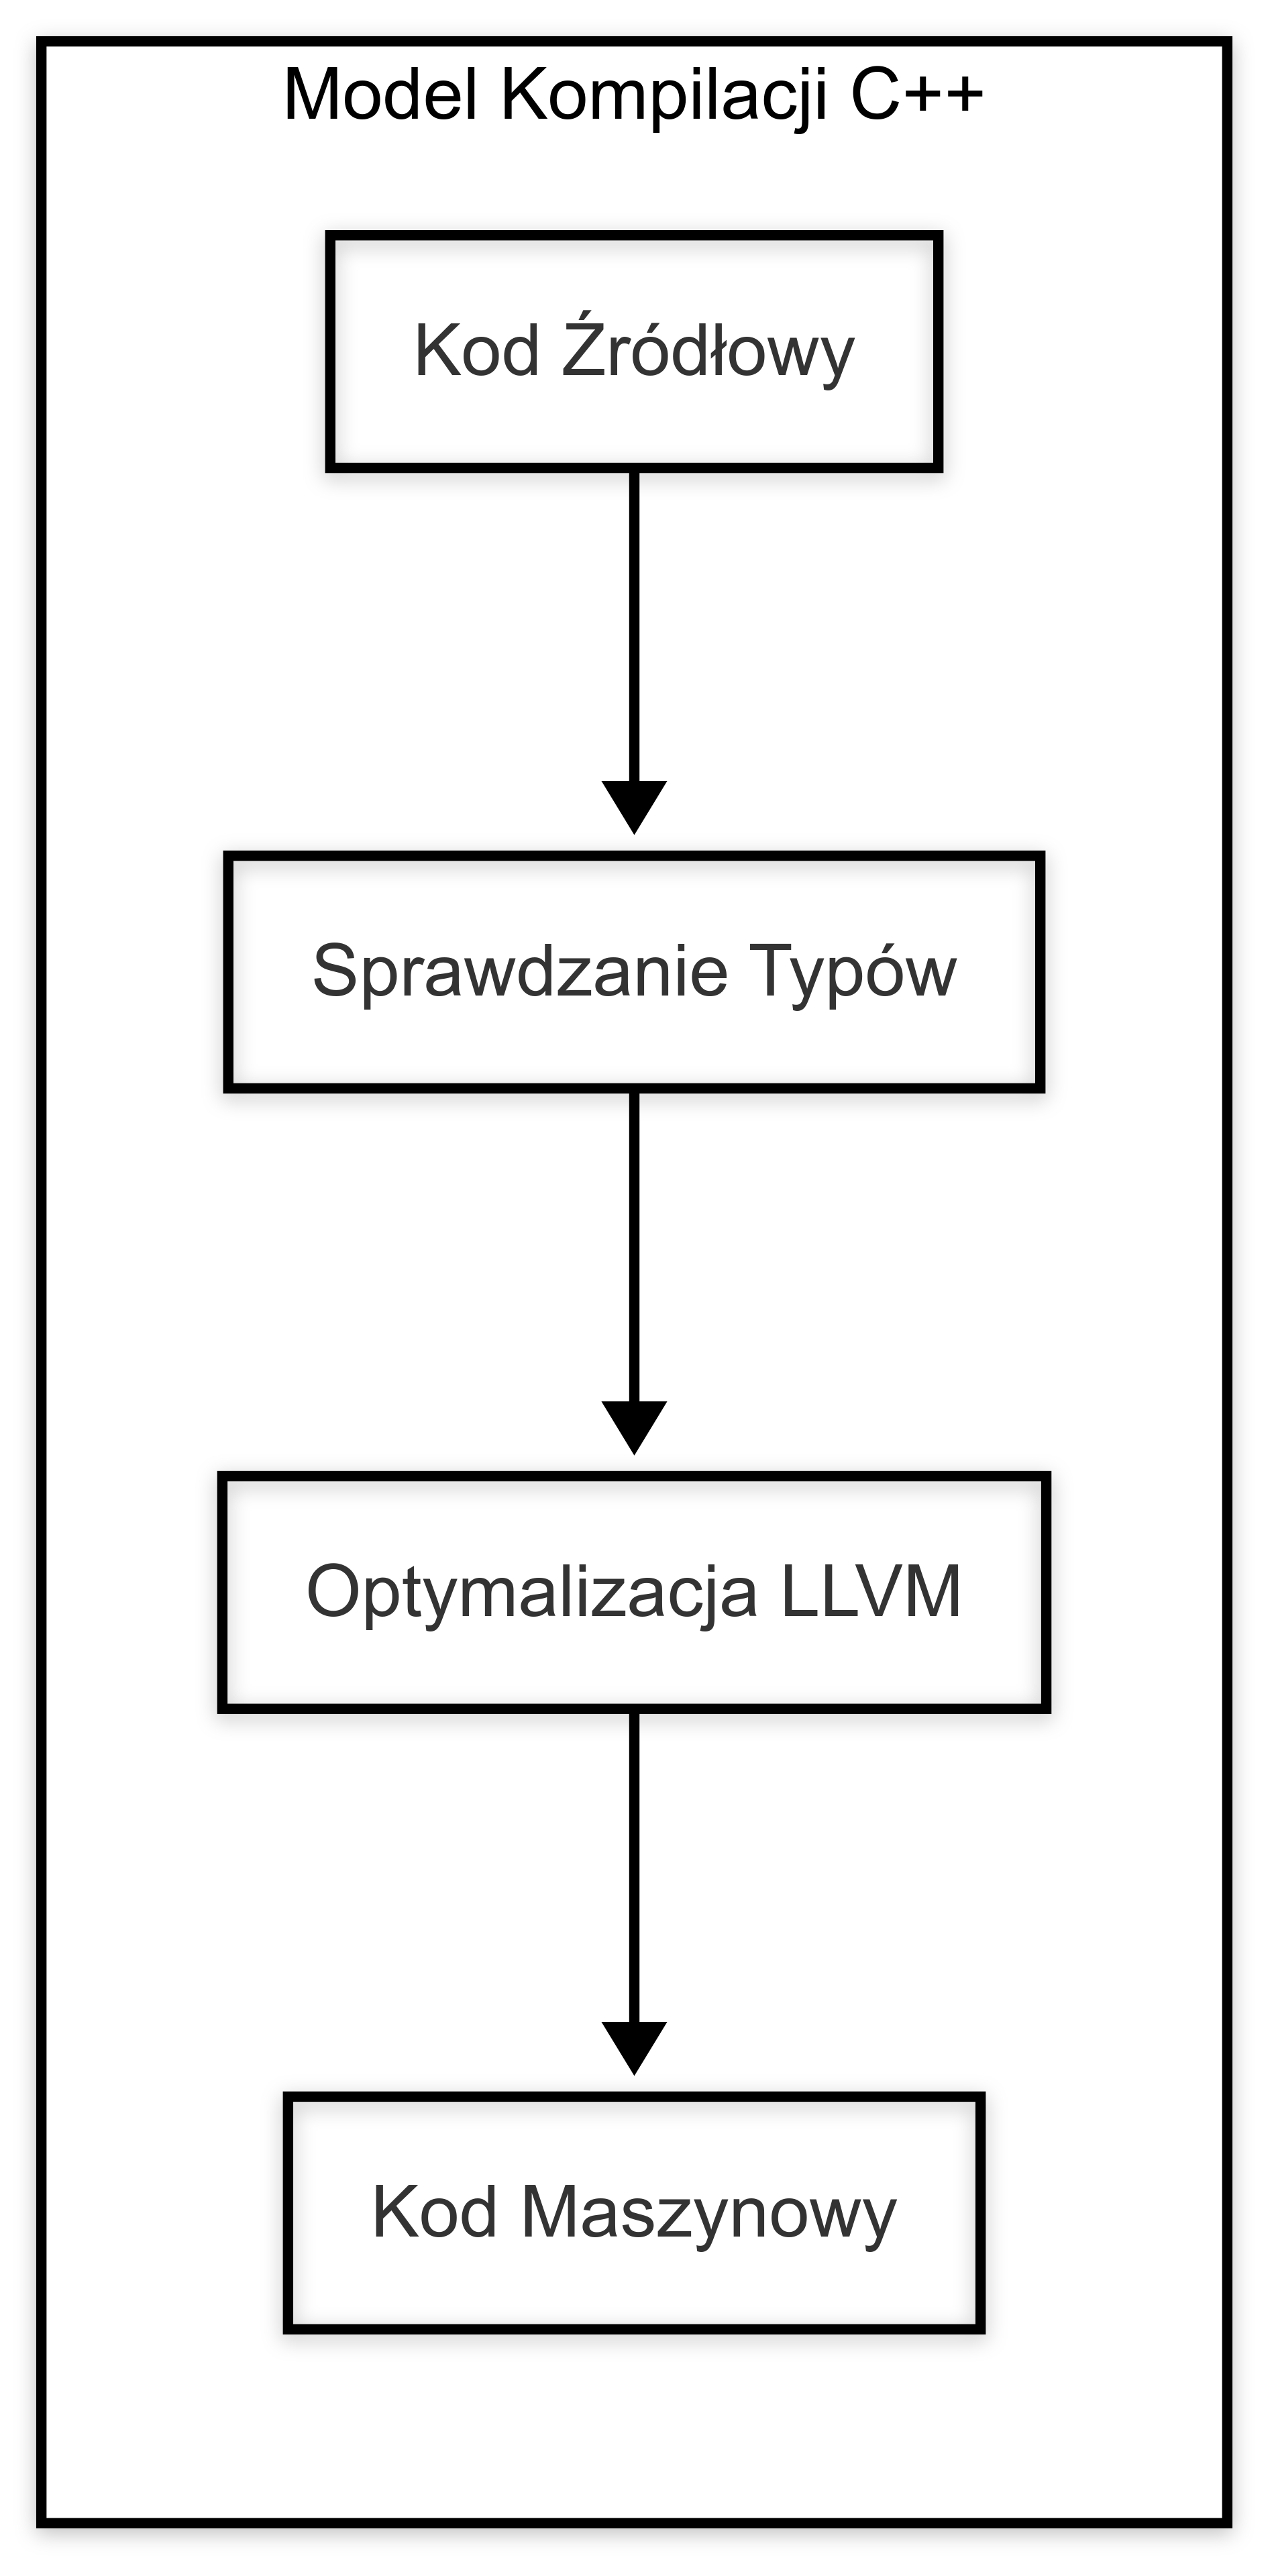
\includegraphics[height=12cm]{images/CppBuildsSteps.png}
        \caption{Kroki kompilacji w języku C++}
        \label{fig:cpp_build_steps}
    \end{minipage}
    \caption{Porównanie kroków kompilacji w językach Rust i C++}
\end{figure}

Informacje o procesie kompilacji pochodzą z \cite{Lesiński, rustPolishNames, TheRustProgrammingLanguage}, które opisują integrację z LLVM i różnice w sprawdzaniu bezpieczeństwa.
Na diagramie \ref{fig:rust_build_steps} drugi blok reprezentuje dodatkowe etapy sprawdzania bezpieczeństwa w Rust, które nie występują w C++. Z kolei na diagramie \ref{fig:cpp_build_steps} drugi blok pokazuje podstawowe sprawdzanie typów w C++, które jest mniej rygorystyczne niż system Rust. Ze względu na różnicę w procesie kompulacji kodu powstają główne różnice w bezpieczeństwie i wydajności obu języków.

C++ nadal pozostaje językiem preferowanym w projektach o krytycznym znaczeniu wydajnościowym, takich jak gry komputerowe, symulacje fizyczne czy systemy wbudowane, choć Rust zaczyna zdobywać popularność w tych obszarach ze względu na większe bezpieczeństwo przy porównywalnej wydajności. 

\subsection{Programowanie współbieżne oraz równoległe}
Współbieżność i równoległość to kluczowe elementy programowania w  językach Rust i C++. Oba języki oferują zaawansowane narzędzia i biblioteki do zarządzania wielowątkowością.

Rust wyróżnia się systemem własności \eng{ownership} i wbudowanym mechanizmem wykrywania błędów współbieżności, co eliminuje wyścigi danych w czasie kompilacji. Narzędzia takie jak Tokio i Rayon pozwalają na łatwe tworzenie i zarządzanie zadaniami asynchronicznymi i równoległymi.
C++ z kolei oferuje wsparcie dla wielowątkowości poprzez standardową bibliotekę (std::thread) oraz zaawansowane szkielety aplikacyjne (frameworks), takie jak OpenMP czy TBB (Threading Building Blocks). Chociaż te narzędzia są niezwykle potężne, nie zapewniają automatycznej ochrony przed błędami współbieżności, co wymaga większej ostrożności ze strony programistów.

Strona \cite{parallelrustcppIntroductionComparing} szczegółowo analizuje różnice w podejściu do współbieżności w obu językach, podkreślając, że Rust dzięki swojemu modelowi zarządzania pamięcią oferuje większe bezpieczeństwo, podczas gdy C++ pozostaje bardziej elastyczny, co może być korzystne w bardziej specyficznych scenariuszach. Jednak jak sam autor \cite{parallelrustcppIntroductionComparing} wskazuje, należy zwrócić uwagę, że większość sztuczek optymalizacyjnych pokazanych w tym porównaniu to jedynie adaptacje oryginalnych rozwiązań C++ w języku Rust. Koncentruje się ona na praktycznym porównaniu języków Rust i C++ pod względem równoległego przetwarzania, szczególnie na poziomie niskopoziomowych operacji i synchronizacji wątków. Znajdują się tam benchmarki pokazujące różnice w czasie wykonywania programów, narzędzia diagnostyczne oraz zestawienie wydajności w kontekście SIMD, wątków, oraz komunikacji międzypamięciowej.

W odniesieniu do artykułów, czasopism oraz materiałów konferencyjnych opublikowanych w latach 2012 \footnotemark-2024, zidentyfikowanie prac, które jednoznacznie koncentrują się na problematyce pracy, jest wyzwaniem. Można natomiast znaleźć publikacje, które wykorzystują wspomniane języki (Rust oraz C++) i ich porównanie w kontekście złożonym do problemu pracy - chociażby wykorzystanie języka Rust w programowaniu układów wbudowanych \cite{ZamiennikWEmbedded}, jako zamiennik dla dotychczasowych języków z rodziny C.\\
Można również znaleźć pracę, która przedstawia wykorzystanie biblioteki odpowiedzialnej za współbieżność FastFlow przez oba języki Rust oraz C++ \cite{FastFlow}. Pokazuje ona, że język Rust jest dobrą alternatywą dla języka C++ w kontekście współbieżności.
\footnotetext{Rust został zaprezentowany w 2012 roku \cite{wikipediaRustprogramming}, a C++ w 1985 roku \cite{wikipediaWikipedia}.}


\section{Podsumowanie}
Na podstawie przeglądu literatury oraz zadanych pytań do przeglądu literatury można wskazać na następujące odpowiedzi
\subsubsection{PPL1: Jakie główne koncepcje/teorie dominują w literaturze dotyczącej porównania języków Rust oraz C++?}
W literaturze dominują badania porównawcze bezpieczeństwa, wydajności oraz zarządzania pamięcią w językach Rust i C++ \cite{PPL1_1} - szczegółowo opisane w podrozdziałach \ref{Bezpieczeństwo} oraz \ref{CzasWykonania}. W kontekście współbieżności i równoległości brakuje systematycznych analiz porównawczych.

\subsubsection{PPL2: Jakie metody badawcze są najcz
ęściej stosowane do analizy różnic pomiędzy językami ?}
W literaturze oraz w dotychczasowych analizach \cite{LanguageComparison_1,LanguageComparison_2,LanguageComparison_3,LanguageComparison_4} wskazano szereg kryteriów istotnych przy porównywaniu lub ocenie języków programowania ogólnego przeznaczenia. Do najważniejszych należą: 
    \begin{itemize}
        \item Prostota konstrukcji języka, mająca bezpośredni wpływ na łatwość programowania i zrozumiałość kodu
        \item Czytelność kodu, związana z jego późniejszą konserwacją i rozwijaniem
        \item Dostosowanie języka do konkretnego zastosowania, co wpływa na wydajność i efektywność programów
        \item Szybkość kompilacji
        \item Efektywność działania programu, zarówno pod względem szybkości, jak i zużycia zasobów systemowych,
        \item Dostępność i jakość bibliotek, frameworków oraz narzędzi wspierających rozwój oprogramowania
        \item Wsparcie w procesie debugowania, profilowania i testowania kodu
        \item Bezpieczeństwo języka, związane z eliminacją błędów w czasie kompilacji oraz wykrywaniem zagrożeń w trakcie działania programu
        \item Długowieczność języka oraz narzędzi kompilacyjnych, co wpływa na stabilność i przewidywalność rozwoju oprogramowania
        \item Przenośność między różnymi platformami i architekturami sprzętowymi.
    \end{itemize}
    Wszystkie te kryteria mają istotny wpływ na całkowity koszt i nakład pracy związany z tworzeniem oraz utrzymaniem oprogramowania, a także na jego jakość i przydatność w długim okresie użytkowania.

    Doświadczenie wskazuje również, że te same kryteria można stosować do oceny innych komponentów wspomagających proces tworzenia oprogramowania, takich jak biblioteki klas obiektowych czy projekty typów abstrakcyjnych. Wykorzystanie odpowiednich, zewnętrznych komponentów oraz dobrze zaprojektowanych rozwiązań przyczynia się do poprawy czytelności, utrzymywalności i ogólnej jakości kodu, jednocześnie przyspieszając proces jego tworzenia.

\subsubsection{PPL3: Jak wygląda porównanie dostępności i dojrzałości bibliotek do programowania współbieżnego i równoległego w obu językach?}
Porównując dostępność i dojrzałość bibliotek do programowania współbieżnego i równoległego w językach Rust i C++, zauważyć można istotne różnice wynikające zarówno z historii rozwoju tych języków, jak i ich podejścia do bezpieczeństwa, abstrakcji oraz zarządzania zasobami.

W przypadku języka C++, biblioteki takie jak OpenMP, Intel TBB czy pthreads cechują się dużą dojrzałością oraz szerokim zastosowaniem w przemyśle, zwłaszcza w kontekście obliczeń naukowych, symulacji fizycznych i systemów o wysokiej wydajności. Są one dobrze udokumentowane, posiadają wsparcie komercyjne (np. TBB) oraz charakteryzują się dużą kompatybilnością z istniejącą infrastrukturą sprzętową i programową. Niemniej jednak, wymagają od programisty głębokiej wiedzy w zakresie zarządzania pamięcią oraz synchronizacji, co przekłada się na wyższy próg wejścia i podatność na błędy (np. wyścigi danych czy zakleszczenia).

Z kolei Rust, jako język nowszy, oferuje bardziej nowoczesny zestaw narzędzi do programowania równoległego, w tym biblioteki takie jak Tokio, Rayon czy Crossbeam. Mimo mniejszej liczby lat rozwoju, biblioteki te szybko dojrzewają i zdobywają popularność dzięki silnym gwarancjom bezpieczeństwa pamięci na poziomie kompilatora oraz ergonomicznemu API. Rust promuje bezpieczne podejście do współbieżności poprzez system własności \eng{ownership} i brak domyślnego współdzielenia zasobów, co w praktyce eliminuje całą klasę błędów typowych dla C++. Dzięki temu biblioteki w Rust, choć mniej rozpowszechnione w starszych zastosowaniach, zyskują przewagę w projektach tworzonych od podstaw, zwłaszcza w środowiskach wymagających wysokiej niezawodności.

\subsubsection{PPL4: Czy istnieją systematyczne metodologie porównywania języków programowania w kontekście problemu pracy, które można zastosować do analizy Rust i C++?}
W literaturze istnieje ograniczona liczba systematycznych metodologii porównujących języki programowania pod kątem programowania współbieżnego i równoległego. Większość badań koncentruje się na analizie wydajności i bezpieczeństwa, nie przyjmując jednolitego podejścia metodologicznego.\\
W ramach porównania mechanizmów równoległości w obu językach, opisanych na stronie \cite{parallelrustcppIntroductionComparing} zastosowano konteneryzację obrazu programu a nastęonie uruchmoenie go na maszynie testowej. Jednak jak podaje arytkuł na stronie Medium \cite{rainbow} może to prowadzić do nie uwzględnienia wpływu takich czynników jak czas uruchamiania, rozmiar obrazu i zużycie pamięci. Podaje również metodę \textit{Rainbow}, która testuje przepustowość, uruchamiając kontenery na podobnej infrastrukturze i używając licznika Redis do śledzenia obliczeń.

\subsubsection{PPL5: Jakie aspekty programowania współbieżnego i równoległego w Rust i C++ nie zostały dostatecznie zbadane w literaturze?}
badania skupiały się przede wszystkim na ogólnych aspektach porównawczych bezpieczeństwa pamięci, zarządzania zasobami oraz wydajności kompilacji i wykonania w językach Rust i C++. Niemniej jednak, istnieją wyraźne luki badawcze, które wymagają pogłębionej analizy, w tym
\begin{itemize}
    \item Systematyczne porównanie specyficznych mechanizmów synchronizacji i zarządzania wątkami, takich jak mutexy, semafory, bariery czy kanały komunikacyjne. Brakuje kompleksowych studiów empirycznych, które umożliwiłyby ocenę efektywności oraz narzutu związanych z implementacją tych mechanizmów w obu językach.
    \item Niedostatecznie zbadany wpływ przyjętych modeli programowania współbieżnego i równoległego na skalowalność i stabilność systemów wielowątkowych, szczególnie w kontekście aplikacji o wysokiej konkurencyjności oraz dynamicznie zmieniających się obciążeń.
    \item Ograniczona liczba badań eksperymentalnych, które wykorzystują benchmarki do porównania realizacji konkretnych konstrukcji językowych (np. asynchroniczności, operacji atomowych) w Rust i C++. Taka analiza mogłaby uwzględniać zarówno aspekty wydajnościowe, jak i bezpieczeństwa wykonywania.
\end{itemize}


\subsubsection{PPL6: Jaki jest stan wiedzy na temat wykorzystania programowania współbieżnego w ramach GPU w językach Rust i C++?}
W literaturze przedmiotowej oraz w praktyce programistycznej, zagadnienie wykorzystania programowania współbieżnego na GPU ewoluuje w różnym tempie w zależności od języka programowania. W przypadku języka Rust obserwujemy dynamiczny rozwój narzędzi, które umożliwiają wykorzystanie mocy obliczeniowej kart graficznych przy jednoczesnym zachowaniu wysokich gwarancji bezpieczeństwa pamięci i wątków.

Projekty takie jak rust‑gpu \cite{rustgpuRust} dążą do umożliwienia pisania shaderów w języku Rust, oferując podejście, które integruje możliwości GPU z bezpiecznymi konstrukcjami języka. Dokumentacja dostępna na stronie github \cite{rustgpuRust} wskazuje na intensywne prace nad przeniesieniem wielu korzyści wynikających z systemu własności i typowania Rust na środowisko GPU, co może przyczynić się do zmniejszenia ryzyka błędów współbieżności, które są szczególnie krytyczne w obliczeniach równoległych.

Równolegle, biblioteka Vulkano (dostępna m.in. poprzez dokumentację \cite{docsVulkanoRust}) stanowi wysokopoziomowy, bezpieczny interfejs do API Vulkan, które jest standardem w programowaniu GPU. Vulkano umożliwia abstrakcję złożoności niskopoziomowych interfejsów, jednocześnie oferując możliwość pełnego wykorzystania równoległości GPU. W podobnym nurcie znajduje się projekt wgpu, który implementuje standard WebGPU, umożliwiając przenośne aplikacje graficzne i obliczeniowe, a jednocześnie integrując współczesne podejścia do zarządzania zasobami i synchronizacji.

W przeciwieństwie do podejścia Rust, w środowisku C++ dominującym rozwiązaniem jest platforma CUDA, rozwijana i wspierana przez firmę NVIDIA \cite{nvidiaCUDAToolkit}. CUDA oferuje bardzo dojrzały, zoptymalizowany i szeroko stosowany framework, który pozwala na bezpośrednią implementację algorytmów równoległych na GPU. W odróżnieniu od narzędzi rozwijanych dla Rust, CUDA posiada ugruntowaną pozycję w środowisku przemysłowym, co przekłada się na bogatą dokumentację, szerokie wsparcie techniczne oraz liczne biblioteki wspomagające rozwój aplikacji wykorzystujących GPU.

Podsumowując, stan wiedzy dotyczący programowania współbieżnego na GPU w języku Rust znajduje się na etapie intensywnego rozwoju i eksperymentacji, gdzie projekty takie jak rust‑gpu, Vulkano oraz wgpu \cite{wgpuWgpuPortable} pokazują potencjał tego podejścia, zwłaszcza w kontekście bezpieczeństwa i nowoczesnych abstrakcji. Z kolei w C++ platforma CUDA, dzięki swojej dojrzałości oraz szerokiemu wsparciu ze strony przemysłu, pozostaje głównym narzędziem wykorzystywanym do implementacji wysokowydajnych obliczeń równoległych na GPU.

\subsection{Kierunki dalszych badań}
Na podstawie przeglądu literatury oraz odpowiedzi na pytania do przeglądu literatury można wskazać na kilka kierunków dalszych badań w dziedzinie programowania współbieżnego i równoległego w językach Rust i C++:
\begin{itemize}
    \item Systematyczne porównanie mechanizmów współbieżnych i równoległych w językach Rust i C++
    \item Analiza wydajności i bezpieczeństwa konkretnych mechanizmów współbieżnych (np. std::thread vs std::thread w Rust, OpenMP vs Rayon, async w Rust vs futures w C++20)
    \item Badania eksperymentalne z wykorzystaniem benchmarków oraz analizy kodu źródłowego w celu porównania języków Rust i C++ w kontekście współbieżności i równoległości
    \item Analiza wykorzystania programowania współbieżnego w ramach GPU w językach Rust i C++
\end{itemize}
